%!TEX TS-program = xelatex
%!TEX encoding = UTF-8 Unicode
\documentclass[final]{kuee_en}
% \usepackage{endfloat}
% \usepackage[final]{hyperref}

\usepackage{xcolor,graphicx}
\usepackage{subcaption}
\usepackage{sectsty} % change section style
\sectionfont{\noindent\textsc} % indent setting
% \usepackage{paralist}
% \usepackage{booktabs}
\usepackage[T1]{fontenc}
\usepackage{tgbonum}


%%%%%%%%%% Start TeXmacs macros
\newcommand{\mathd}{\mathrm{d}}
\newcommand{\tmname}[1]{\textsc{#1}}
\newcommand{\tmop}[1]{\ensuremath{\operatorname{#1}}}
\newcommand{\tmtextit}[1]{{\itshape{#1}}}
\newcommand{\nosymbol}{}
\newcommand{\tmmathmd}[1]{\ensuremath{#1}}
%%%%%%%%%% End TeXmacs macros


\etitle{Broadband frequency entangled photon generation using silicon nitride ring cavities}
\title{\cjk{窒化シリコン\\リング共振器を用いた\\広帯域周波数もつれ光子生成}}
\eauthor{Zhenghao Yin} 
\author{\cjk{殷 政浩}}
\supervisor{\cjk{竹内 繁樹 教授}}
\school{\cjk{京都大学大学院工学研究科}}
\depart{\cjk{電子工学専攻}}
\date{\cjk{令和2年2月1日}}

\begin{document}
\maketitle

\begin{abstract}
    \lipsum[1]
\end{abstract}

\chapter{Introduction}
\lipsum[2-3]
\chapter{Principal Theory}

In chip scale quantum optical platforms, to confine the light in a sub-micron dimension, the mean how light propagate is different from the TEM mode or Gaussian mode in free space. Based on the conventional guided wave theory, the fundamental mode, which is mainly used in integrated optical applications, can be solved in some simple cases with some approximations. Furthermore, due to the broadband motivation in this study, it is essential to the dispersion into consideration, not only in the part of propagation but also the nonlinear progress where the photon pairs are generated.

In this chapter, the waveguide theory is roughly introduced and sequentially, mode coupling theory is discussed in the case of ring resonator. Second section will focus on nonlinear optics in the view of waveguide.

\section{Guided modes}

In an ideal optical waveguide, the core layer and the cladding layer are usually composed of two different materials, where the refractive index is larger in the core. As an analogue of optical fibers, only in the higher index regime can the light propagate, and meanwhile dissipate in a wavelength scale in the lower index regime.

Usually, we assume the core and the cladding layer are made of nonmagnetic (magnetic permeability $\mu = \mu_0$) and dielectric material (conductivity $\sigma = 0$). Furthermore, we neglect the nonlinear response of the polarization of electric field ($\vb{P} \simeq \varepsilon_0 \chi \vb{E}$).

Since the waveguide in numerous research objects, is deposited or sputtered using chemical or physical methods, the uneven density in the waveguide layer can not be negligible. Hence, the propagation equation derived from Maxwell's equation is
\begin{equation}\label{eq:aniso}
  (\nabla_{\perp}^2 + k^2 n^2 - \beta^2) \vb{E} = - (\nabla_{\perp} + i
  \beta \hat{\vb{z}}) (\vb{E_{\perp}} \nosymbol \cdot \nabla_{\perp} \ln
  n^2)
\end{equation}
where $\perp$ denotes the transverse component, $\nabla_{\perp}^2 = \nabla_x^2 + \nabla_y^2$. And $k, n, \beta$ are the wave vector in vacuum, refractive index and propagation constant, respectively. While, with the negligible film anisotripy, Eqn. \ref{eq:aniso} can be approximated into
\begin{equation}\label{eq:helm}
  (\nabla_{\perp}^2 + k^2 n^2 - \beta^2) \vb{E} = 0
\end{equation}
This is the normal \textit{Helmholtz equation}, indicating the relation between propagation constant $\beta$ and material refractive index, i.e. \textit{chromatic dispersion}.

Next, the boundary conditions determining the solution to Eqn. \ref{eq:helm}, arise from the Maxwell's equations as well.
\begin{eqnarray*}%\label{eq:bcon}
  \vb{\hat{n}} \cdot (\vb{E_a - E_b}) & = & 0 \\
  \vb{\hat{n}} \times (\vb{\vb{H_a} - H_{\vb{b}}}) & = & 0
\end{eqnarray*}
which is the continuity condition of both electric and magnetic field at all dielectric material interfaces. Here, $\vb{\hat{n}}$ is the normal direction at the material boundary and the subscript $a, b$ denote different regimes.

In the case of channel waveguides, the index discontinuity from both vertical and horizontal sides can be decomposed into two sets of independent and complete conditions, i.e. the horizontal boundary condition and vertical boundary condition, with the discontinuity on the waveguide corners neglected. In other words, approximately the equation has two independent partiuclar solutions, which is the mathematical origin of \textit{ transverse electric} (TE) modes and \textit{transverse magnetic} (TM) modes.

\begin{figure}
\centering
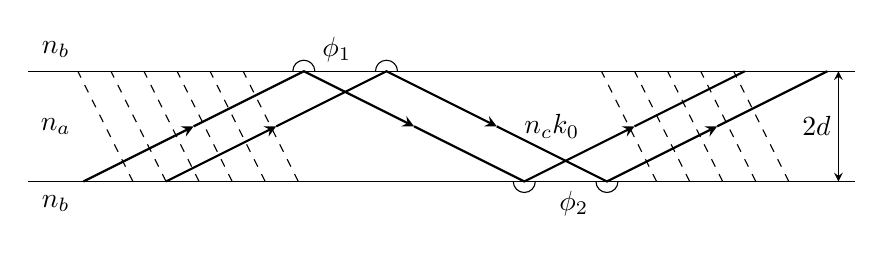
\begin{tikzpicture}[scale=0.7,>=stealth]
\draw (-9,0) -- (6,0) (-9,2) -- (6,2);
% \draw [->] (-9,1) -- (6,1);
\foreach \x in {0,1.5}{
  \draw [thick, ->] (-8+\x,0) -- (-6+\x,1);
  \draw [thick,->] (-6+\x,1) -- (-4+\x,2) -- (-2+\x,1);
  \draw [thick,->] (-2+\x,1) -- (0+\x,0) -- (2+\x,1);
  \draw [thick,-] (2+\x,1) -- (4+\x,2);
}
\foreach \x in {-1,0,1,2,3,4}
	\draw [dashed] (-6.5+0.6*\x,0) -- (-7.5+0.6*\x,2);
\foreach \x in {0,1,2,3,4}
	\draw [dashed] (2.4+0.6*\x,0) -- (1.4+0.6*\x,2);

% \draw [<->] (-9,1.5) --(-9,0.7) -- (-7.4,0.7);
% \draw [->] (-9,0.7) -- (-7.4,1.5);

% \node at (-8.6,1.4) {$\tiny{k_i}$};
% \node at (-8.2,0.4) {$\tiny{\beta}$};
\node at (0.5,1) {$n_c k_0$};

\draw [<->] (5.7,0) -- (5.7,2);
\node at (5.3,1) {$2d$};
\node at (-8.5,1) {$n_a$};
\node at (-8.5,2.4) {$n_b$};
\node at (-8.5,-0.4) {$n_b$};
\node at (-3.4,2.4) {$\phi_1$};
\node at (0.9,-0.4) {$\phi_2$};

\draw (-3.8,2) arc [start angle=0, end angle=180, radius=0.2];
\draw (-3.8+1.5,2) arc [start angle=0, end angle=180, radius=0.2];

\draw (-3.8+3.6,0) arc [start angle=180, end angle=360, radius=0.2];
\draw (-3.8+5.1,0) arc [start angle=180, end angle=360, radius=0.2];

\end{tikzpicture}
\caption{\textbf{Planar waveguide}. The upper}
\label{fig:ch1-planar}
\end{figure}

Hence, we can study the eigenequantion by selecting only one set of boundary condition, as part of \textit{the effective index method}. For example, in a planar waveguide shown in Fig. ,$\dv[2]{}{y}=0$\footnote{Since the planar waveguide is infinite at the $y$-direction , thus the solution is identical in arbitrary $xz$-plane, which means no gradient along $x$-axis.},
the TE mode features $E_x=0$ and consider only $y$-component, 
\begin{equation}
    \dv[2]{E_y}{x} + (k^2 n^2 - \beta^2)E_y =0
\end{equation}
and $E_y$ is continous at $x=\pm d$, where $2 d$ is the thickness of core layer. By substituting this condition, 

\begin{equation}
    2k_x d = m\pi + 2\arctan(\kappa/k_x)
\end{equation}

\section{Ring resonators}

The working principle of ring resonator is derived completely in Ref. \cite{Bogaerts2012}. Like Fabry-P\'{e}rot etalon,  based on the coupling mode theory, the transmission of a all-pass type ring cavity takes the form
\begin{equation}
    T_n = \frac{I_\mathrm{pass}}{I_\mathrm{input}} = \frac{a^2 - 2ar \cos \phi + r^2}{1 - 2ar \cos \phi + a^2 r^2}
\end{equation}
Here $a$ is single-pass amplitude transmission, including the propagation loss in the ring and coupling loss between the bus waveguide and the cavity, $r$ is the self-coupling coefficient, denoting the transmission before and after coupling, $\phi=\beta L$ is the phase shift in a single trip. Given the specific device, the 

\section{Nonlinear optics}

In addition, in the case of nonlinear photonics, the nonlinear response of the
electric field is inherent and essential, hence we also derive the propagation
by treating the nonlinear term as an additive source.



In addition, in the case of nonlinear photonics, the nonlinear response of the
electric field is inherent and essential, hence we also derive the propagation
by treating the nonlinear term as an additive source.

\section{Four wave mixing}


Assume in a ring resonator, to satisfy both energy conservation and momenmtum
conservation,
\begin{eqnarray*}
  \beta_i + \beta_s & = & 2 \beta_p\\
  \omega_i + \omega_s & = & 2 \omega_p
\end{eqnarray*}
meanwhile, $\beta = m \frac{2 \pi}{L}$, and $L$ is the length of the
resonator. Thus,

{\tmname{\begin{equation}
  m_i + m_s = 2 m_p
\end{equation}}}

Hence, \tmtextit{the momenmtum conservation agrees with mode numder
equidistant.} Thus, we choose the frequency domain to estimate the phase
mismatch. Expand the frequency into Taylor seires at $\omega_0$ to the
propagation constant $\beta$,
\begin{eqnarray}
  \omega_{\mu} & = & \omega_0 + \frac{\mathd \omega}{\mathd \beta}
  (\beta_{\mu} - \beta_0) + \frac{1}{2}  \frac{\mathd^2 \omega}{\mathd
  \beta^2} (\beta_{\mu} - \beta_0)^2 + \cdots \\
  & = & \omega_0 + \frac{\mathd \omega}{\mathd \beta} \frac{2 \pi}{L} \mu +
  \frac{\mathd^2 \omega}{\mathd \beta^2} \left( \frac{2 \pi}{L} \mu \right)^2
  + \cdots \nonumber\\
  & = & \omega_0 + D_1 \mu + D_2 \mu^2 + D_3 \mu^3 + \cdots \nonumber
\end{eqnarray}
where $D_1 / 2 \pi = 1 / v_g L$ is the \tmtextit{free spectrum range}, and
\begin{eqnarray*}
  \tmop{as} & = & a
\end{eqnarray*}

\bibliography{library}
\bibliographystyle{abbrv}

\end{document}
